\headline{{\textbf{\Large\sffamily TWBC Club Events:}}\\
          {\textbf{\large\sffamily Trees of the Month \& Workshops}}}
\label{2025-10-calendar}
\noindent
Just a gentle reminder for the Tree of the Month themes and workshops organised by our club throughout the year.

\textbf{Note:} We encourage new members to participate in the \textit{Novice Tree of the Month Table}.
This can be any species of tree and is intended to help newer members (under two years with the club) gain experience in presentation and display.  
The voting format is the same as for the main table, and certificates will be awarded to the winner at the end of the evening.

\medskip
\noindent
\textbf{Important Update for November 2025:}
Please note that due to a change in availability, \textit{David Cheshire} will now visit the club later in November.  
The \textbf{AGM} will take place on \textbf{13th November}, and the \textbf{Club Evening with David Cheshire} will now be held on \textbf{27th November}.
We hope this change will allow everyone to attend both events and enjoy David's demonstration and talk.

\medskip
\topic{November 2025}
\begin{itemize}
    \item \textbf{13th November:} \textit{Annual General Meeting (AGM)}
    \item \textbf{27th November:} \textit{Club Evening with \textit{David Cheshire} – Demonstration and Talk}
    \item \textbf{Tree of the Month:} \textit{Any tree previously submitted for Tree of the Month during the year.}
\end{itemize}

\medskip
\topic{December 2025}
\begin{itemize}
    \item \textbf{Workshop of the Month:} \textit{Festive fun \& Party time!}
\end{itemize}

\medskip
\noindent
\textbf{Note:} The Tree of the Year is \textit{Elm}.
\closearticle

\vfill
\begin{center}
	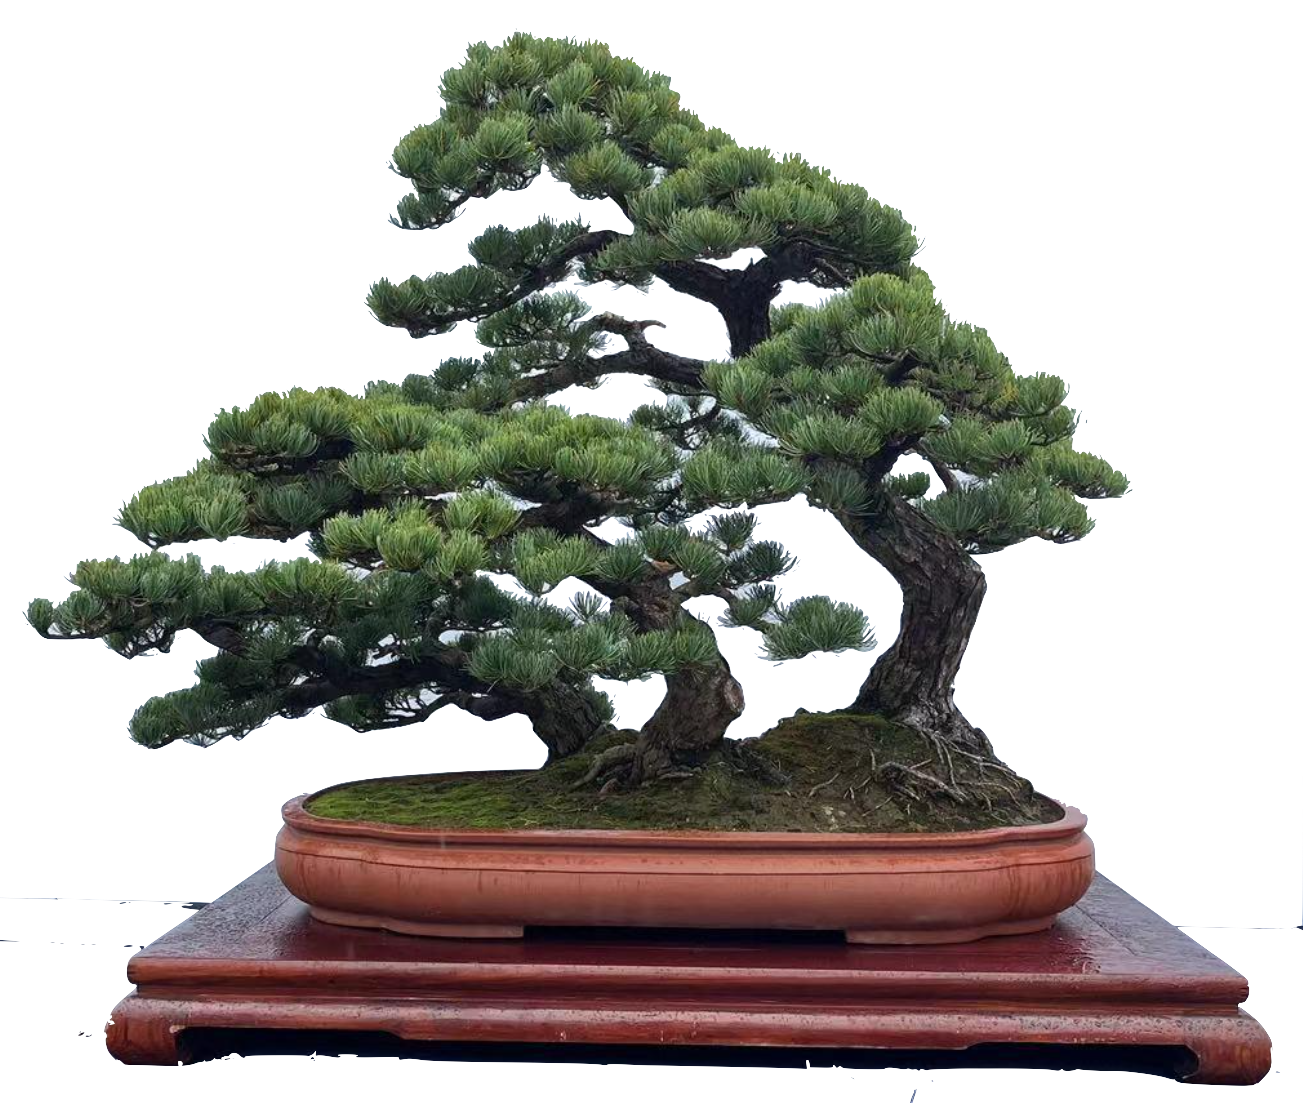
\includegraphics[width=0.75\columnwidth]{res/filler_a}
\end{center}
\columnbreak
